\chapter{FHP}
This improved lattice gas cellular automaton is named after its inventors too -- Frisch, Humpfrey and Pomeu. 
They proposed it in 1986 together with its three dimensional variant - the FCHC. 
%Comparing it to HPP, we have a lattice with better rotational symmetry and nodes with richer  set of collisions.
%
Now that we presented the setting of FHP in two dimensions rather intuitively, let us explore the microdynamics of FHP in a more formal way. The formal treatment provides that the hydrodynamic equations that we derive are valid for FHP in arbitrary dimension (although finding an appropriate multidimensional lattice is non-trivial and possible only in 4 dimensions, as we will see).
In following section, we will graphically explain the basic principles of FHP, the other sections will be more general and the obtained results will be valid for arbitrary dimensional FHP-like automaton (most importantly FCHC).

\section{The lattice of FHP}
All the improvements of FHP are result of one simple change - instead of square grid, FHP builds on hexagonal grid. All other properties are implied by its hexagonal layout.
%
%The two dimensional plane can be uniformly covered by squares, but also by hexagon, that . This is the main improvement of FHP, all other properties are implied by the properties of the hexagonal grid.

On the figure \ref{FHPgrid}, we have a part of hexagonal grid, and from one of the node, six lattice vectors points to the neighboring nodes.
Let us denote the set of these vectors by $c_i,~i=1,2,3,4,5,6$.


\begin{figure}[htbp] \label{FHPgrid}
 \centering
 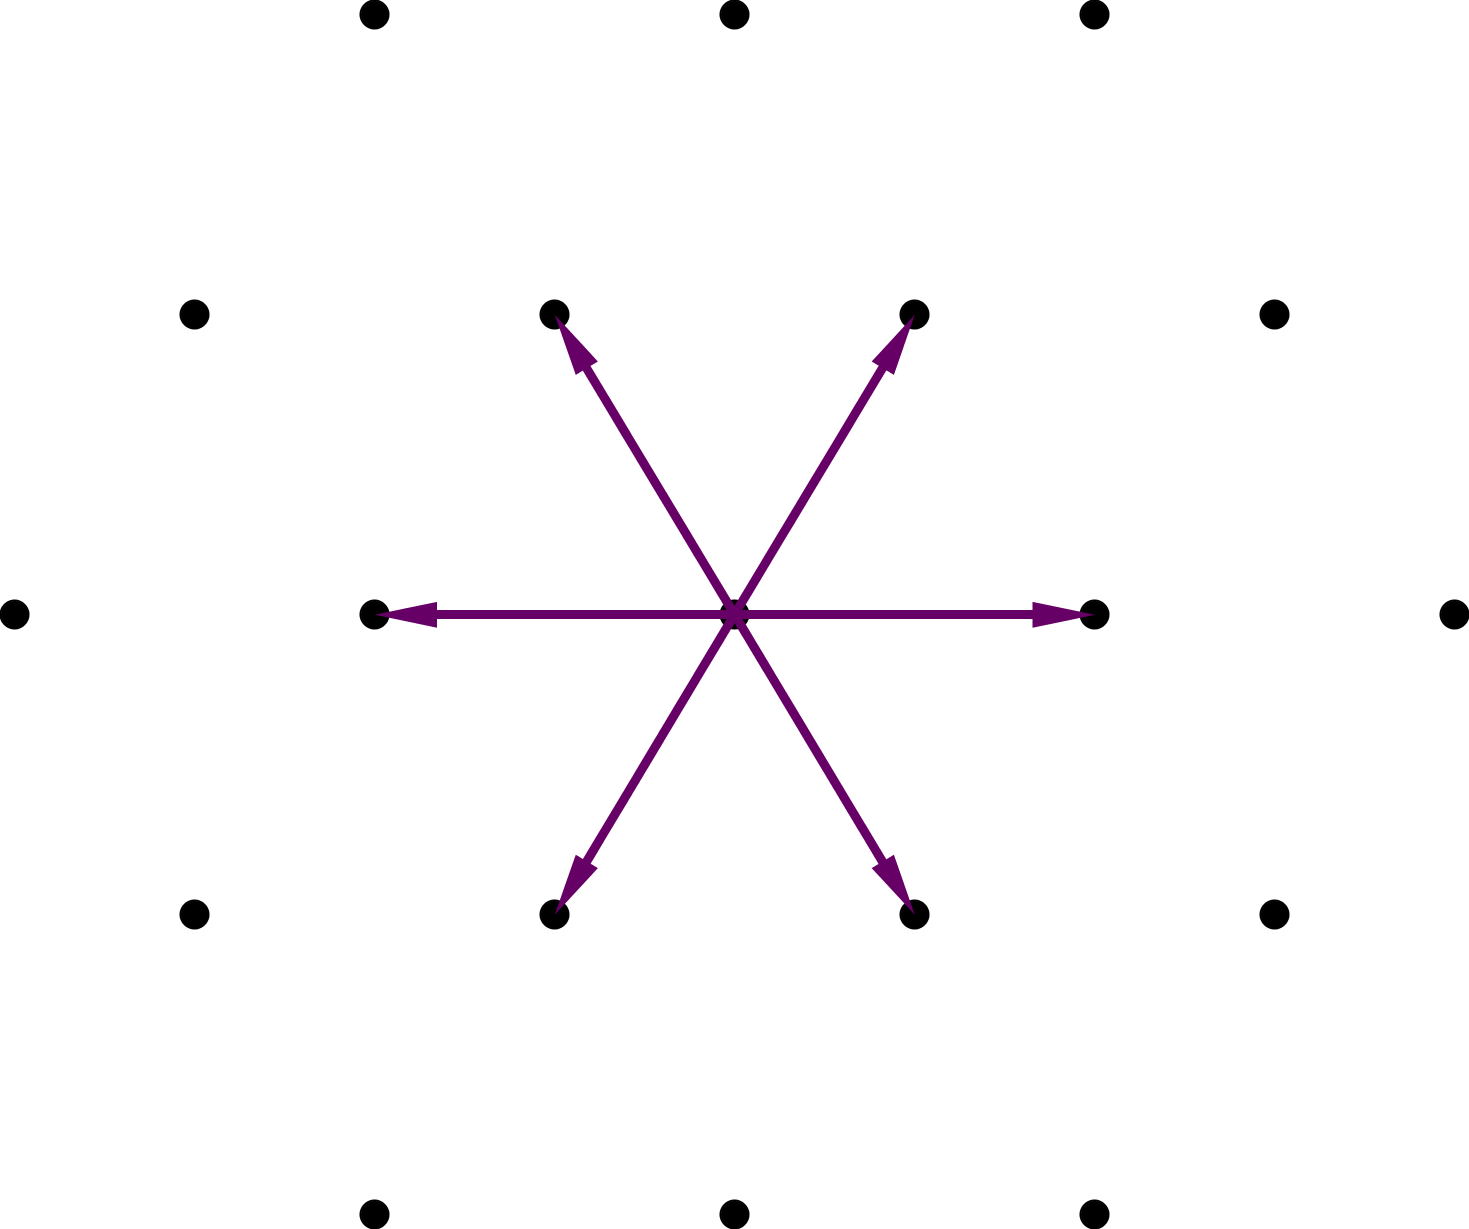
\includegraphics[width=0.6\textwidth]{./img/fhp_desc}
\end{figure}

To each of these vectors, there is corresponding cell in the node.
The node is nothing else then a set of the six cells.
Let us denote the state of the node by $\bm{n} = (n_1,n_2,n_3,n_4,n_5,n_6)$, where $n_i = 0$ stands form empty $i^{th}$ cell, and $n_i = 1$ implies that there is a particle in the $i^{th}$ cell. 

State of a node with the position $\bf{r}$ on lattice will be denoted by $\bf{n(r)}$, whereas the state of the \textit{whole lattice} will be denoted by \textbf{n(.)}.

\section{Update rule}
As we know, the update happens in discrete time steps ($t=1,2,3...$) and consists of two subsequent steps - collision and propagation. Both of these steps are local, so they can be treated node by node.

\subsection{Propagation}

Propagation is the straight-forward phase and can be captured by the simple equation
\begin{align*}
S n_i(\bf{r}) = n_i(\bf{r + c_i}). 
\end{align*}
%This equation means that state of the $i^{th}$ cell in node \textbf{n(r)} \textit{propagates} along the lattice vector $c_i$ to the neighboring node $\bf{n(r + c_i)}$, the figure \ref{FHPprop}.
If the cell is occupied by a particle ($n_i(\bf{r})=1$), it propagates along the corresponding lattice vector to the neighboring node, see the figure \ref{FHPprop}.

The propagation, however, is preceded by the more interesting step -- the collision.

\subsection{Collision}

The purpose of the collision is to swap as many particles in the node as possible.
The only constraint on the collision rule is to preserve the number of particles (conservation of the mass) and to preserve the total momentum in the node (conservation of the momentum).
These requirements lead only to a handful of collision configurations, see figure \ref{FHPcol}. For the simplicity, we are considering the FHP-I model, that does not included the "rest particles", otherwise we would have to add few more collisions.

\begin{figure}[H]
 \centering
 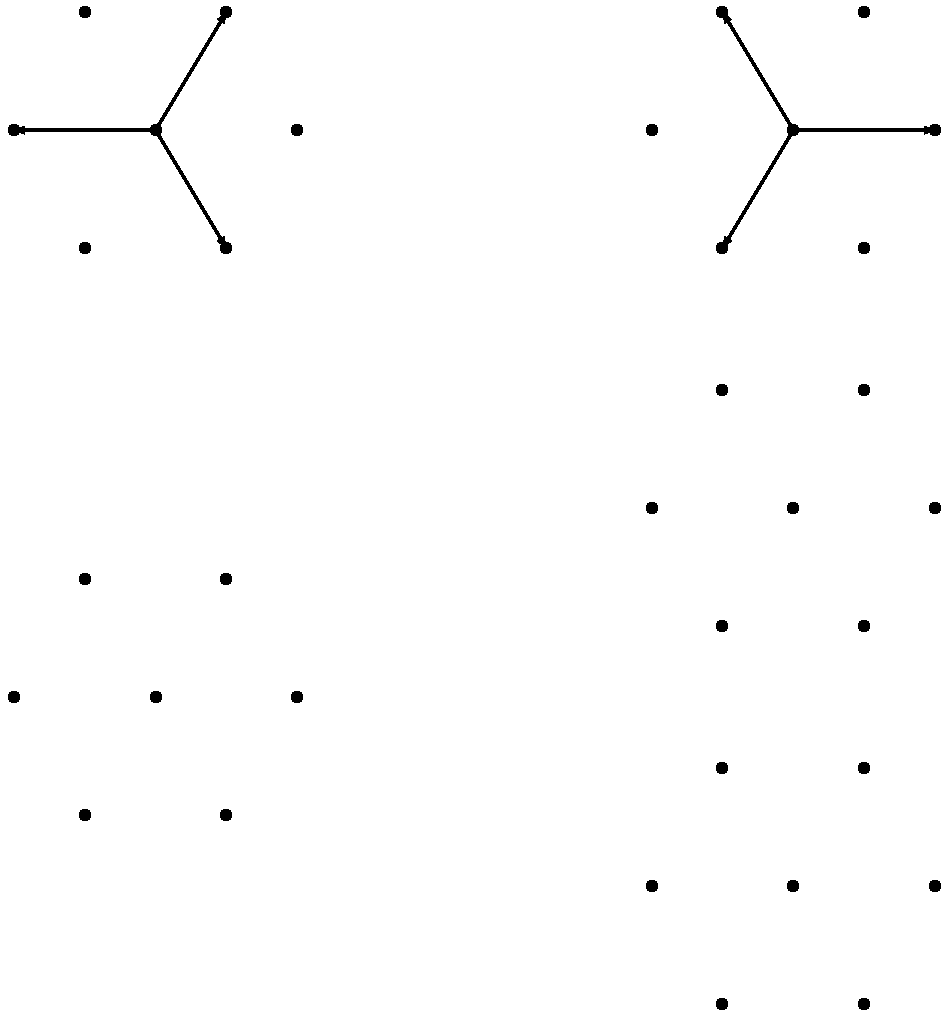
\includegraphics[width=0.7\textwidth]{./img/FHPcol}
 \caption{FHP collisions without rest particle.}
 \label{FHPcol}
\end{figure}

We see that two and four particle configurations can be resolved in two different configurations. The resulting state need to be chosen randomly, with probability $1/2$ for each state to preserve the parity symmetry of the model. If we were systematically choosing only one of them, we would introduce additional, non-physical invariant - chirality. Hence, we need to introduce non-determinism to the model.


We will express the probabilities of transition from state $n$ to state $n'$ by probability matrix:
\begin{equation}
A(n \rightarrow n') \geq 0
\end{equation}
As we have 64 possible states of the node, matrix A is of dimension $64\times 64$.
For example, the cell of matrix A that governs the head-on collisions looks like this:
\[
 A'=
  \begin{bmatrix}
    0 & \frac{1}{2} & \frac{1}{2} \\
    \frac{1}{2} & 0 & \frac{1}{2} \\
    \frac{1}{2} & \frac{1}{2} & 0 \\
  \end{bmatrix}
\]
Since the collisions are symmetric, matrix A is symmetric as well.

Also, collisions are invariant to rotations or reflections of the node:
\begin{equation}
A(g(n) \rightarrow g(n')) = A(n \rightarrow n')
\end{equation}
where $g \in G$, and G is the symmetry group of the node.


\section{Collision operator}
Interestingly, we can express the whole update step in one simple equation using collision operator $\Delta_i$:
\begin{equation}
n_i(t+1,r+c_i) = n_i(t,r) + \Delta_i(t,r)
\end{equation}
If this equation works, then, $\Delta_i$ must be:
\begin{enumerate}
\item $\Delta_i = 0$ if no collision is happening in $n(t,r)$. Then state of the cell $n_i(t,r)$ only propagates to $n_i(t+1,r+c_i)$.
\item $\Delta_i = 1$ if there is not particle in $n_i(t,r)$ yet, but gets there after collision. 
 \item $\Delta_i = -1$ if there is particle in the $n_i(t,r)$, but after collision, cell gets empty.
\end{enumerate}

\bigskip

For example, $\Delta_i$ acquire very simple form for HPP:
\begin{equation}
\Delta_i = n_{i+1} n_{i+3}( 1 - n_i)(1 - n_{i+2}) - n_i n_{i+2}(1-n_{i+1})(1 - n_{i+3})
\end{equation}
As there are only 2 collision configuration in HPP, $\Delta_i$ has 2 terms.
If either collision happens, corresponding term is 1.

\section{Microscopic conservation laws}
Using collision operator, conservation of mass and momentum is this simple:
\begin{subequations}
\begin{align}
\sum_i \Delta_i(t,r) &= 0,\\
%
\sum_i c_i \Delta_i(t,r) &= 0
\end{align}
\end{subequations}
(Prove: unfold $\Delta$s)
Conservation laws can be equivalently expressed in the form
\begin{align} \label{cons1}
\begin{split}
\sum_i n_i(t+1, r + c_i) &= \sum_i n_i(t,r), \\
\sum_i c_i n_i(t+1, r + c_i) &= \sum_i c_i n_i(t,r).
\end{split}
\end{align}


%
%When the collision is resolved in every node, propagation follows.
%This phase is straigt-forward -- 
%
%\begin{figure}[H]
% \centering
% 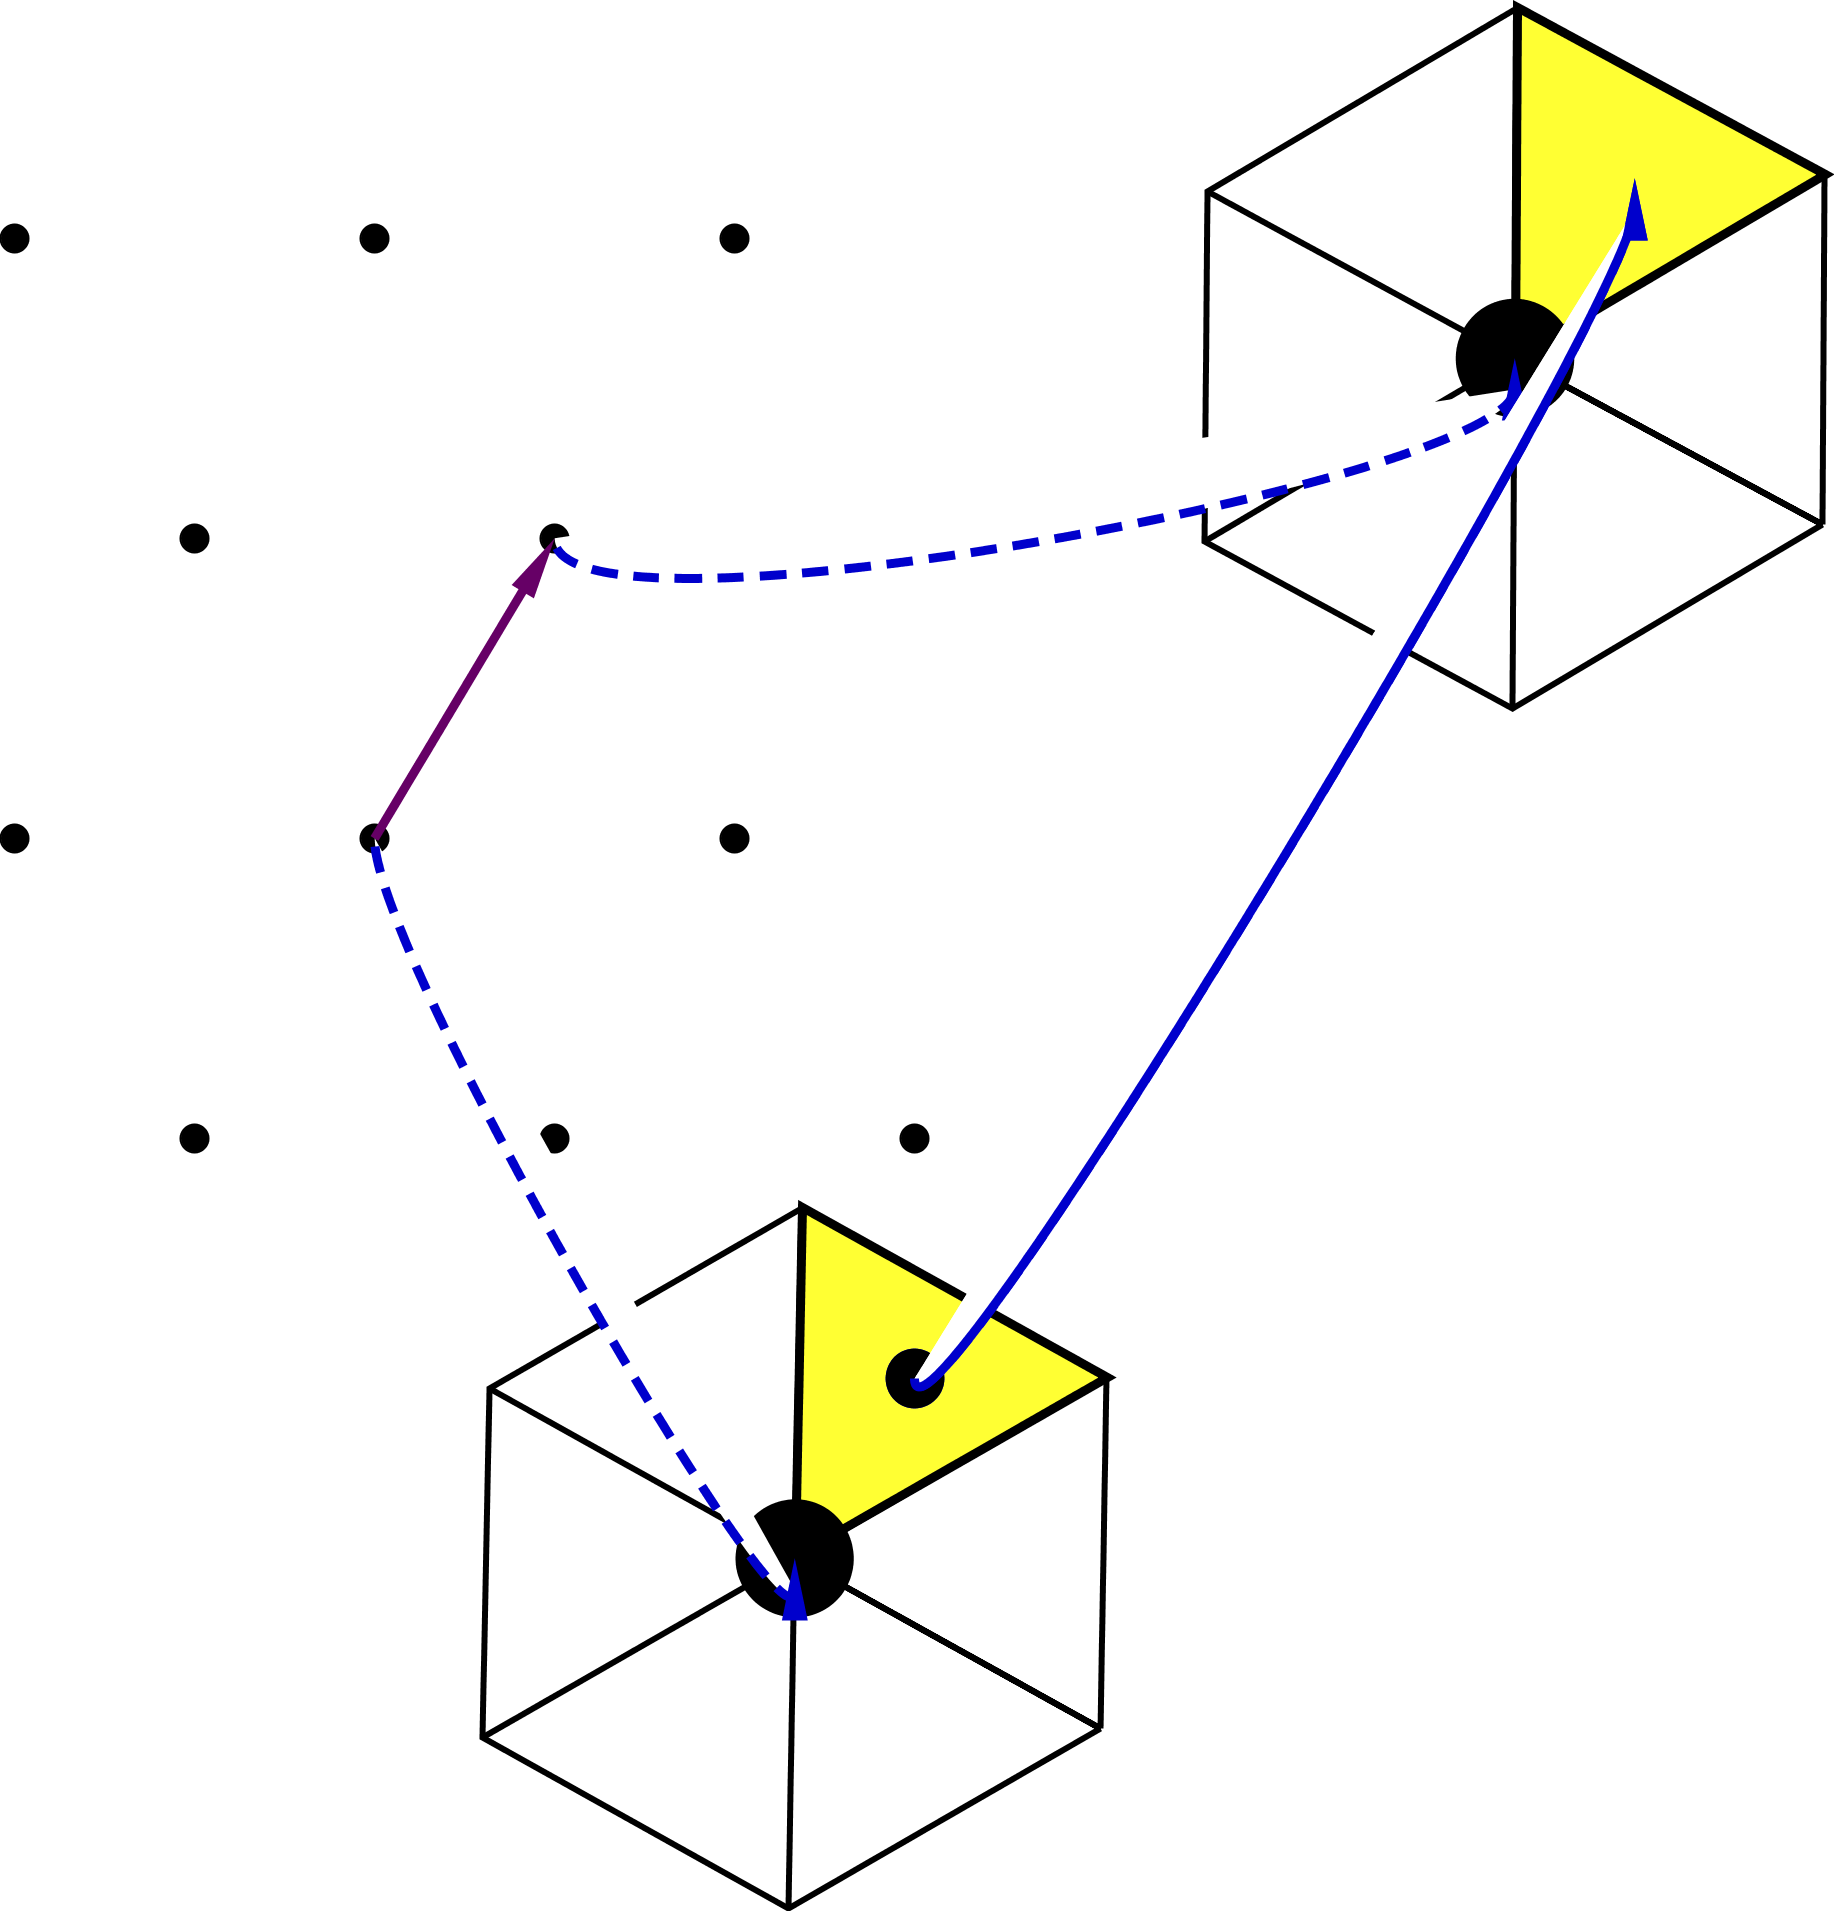
\includegraphics[width=0.7\textwidth]{./img/FHPprop}
% \caption{FHP collisions without rest particle.}
% \label{FHPprop}
%\end{figure}



%Therefore, every node consists of the six cells corresponding to these lattice vectors.
 
%Let us denote the state of the node by $\bm{n} = (n_1,n_2,n_3,n_4,n_5,n_6)$, where $n_i = 0$ stands form empty $i^{th}$ cell, and $n_i = 1$ implies that there is a particle in the $i^{th}$ cell.
% 
%We can actually identify lattice velocities of the particles with lattice vectors, as we are free to set their norm to be the same.
%
%\section{Update rule}
%In all LGCAs, the update of the lattice happens in discrete time steps and consists of two subsequent steps - collision and propagation. Both of these steps are local, so they can be treated node by node.
%
%and will be denoted by $t=1,2,3...$ and so forth. Update can be divided in two subsequent steps - collision and propagation. Both of these steps are local, so they can be treated node by node.

%The purpose of the collision is to swap as many particles in the node, as conservation of mass and momentum allows. This leads to the desirable minimization of viscosity.

%The only constraint on the collision rule is to preserve the number of particles (conservation of mass) and to preserve the total momentum in the node (conservation of momentum).

%
%Comparing it to HPP, we have a lattice with better rotational symmetry and nodes with richer  set of collisions.
%
%Now that we presented the setting of FHP in two dimensions rather intuitively, let us explore the microdynamics of FHP in a more formal way. The formal treatment provides that the hydrodynamic equations that we derive are valid for FHP in arbitrary dimension (although finding an appropriate multidimensional lattice is non-trivial and possible only in 4 dimensions, as we will see).
%
%\section{Convention that we will use}
%State of the node will be denoted by $\bm{n} = (n_1,n_2,n_3,n_4,n_5,n_6)$, where $n_i = 0$ stands for the empty $i^{th}$ cell, and $n_i = 1$ implies that there is a particle in the $i^{th}$ cell.
%
%State of a node with the position $\bf{r}$ on lattice will be denoted by $\bf{n(r)}$, whereas the state of the \textit{whole lattice} will be denoted by \textbf{n(.)}.
%
%As we know, the update happens in discrete time steps that we will denote by $t=1,2,3...$ and so forth.
%
%\section{Propagation}
%Propagation is the straight-forward step and can be captured by the simple equation
%\begin{align*}
%S n_i(\bf{r}) = n_i(\bf{r + c_i}). 
%\end{align*}
%This equation means that state of the $i^{th}$ cell in node \textbf{n(r)} \textit{propagates} along the lattice vector $c_i$ to the neighboring node $\bf{n(r + c_i)}$, the figure \ref{FHPprop}.
%
%\section{Collision}
%As we already sketched, the purpose of the collision is to swap as many particles in the node, as conservation of mass and momentum allows.
%
%For FHP in two dimensions, we have $2^6 = 64$ configurations, and whole bunch of collision configurations among them (figure \ref{FHPcol}).

%
%As we see, head-on 2-particle collisions and 4-particle collisions can result in two different states. If we wanted to preserve determinism, and we were systematically choosing only one of them, we would introduce additional, non-physical invariance - the model would become chiral. If we want to preserve the parity symmetry of the model, we need to assign equal probability to either of two final states.Hence, we are introducing non-determinism to the model.
%
%We will express the probabilities of transition from state $n$ to state $n'$ by probability matrix:
%\begin{equation}
%A(n \rightarrow n') \geq 0
%\end{equation}
%As we have 64 possible states of the node, matrix A is of dimension $64\times 64$.
%For example, the cell of matrix A that governs the head-on collisions looks like this:
%\[
% A'=
%  \begin{bmatrix}
%    0 & \frac{1}{2} & \frac{1}{2} \\
%    \frac{1}{2} & 0 & \frac{1}{2} \\
%    \frac{1}{2} & \frac{1}{2} & 0 \\
%  \end{bmatrix}
%\]
%Since the collisions are symmetric, matrix A is symmetric as well.
%
%Also, collisions are invariant to rotations or reflections of the node:
%\begin{equation}
%A(g(n) \rightarrow g(n')) = A(n \rightarrow n')
%\end{equation}
%where $g \in G$, and G is the symmetry group of the node.

%\section{Collision operator}
%Interestingly, we can express the whole update step in one simple equation using collision operator $\Delta_i$:
%\begin{equation}
%n_i(t+1,r+c_i) = n_i(t,r) + \Delta_i(t,r)
%\end{equation}
%If this equation works, then, $\Delta_i$ must be:
%\begin{enumerate}
%\item $\Delta_i = 0$ if no collision is happening in $n(t,r)$. Then state of the cell $n_i(t,r)$ only propagates to $n_i(t+1,r+c_i)$.
%\item $\Delta_i = 1$ if there is not particle in $n_i(t,r)$ yet, but gets there after collision. 
% \item $\Delta_i = -1$ if there is particle in the $n_i(t,r)$, but after collision, cell gets empty.
%\end{enumerate}
%
%\bigskip
%
%For example, $\Delta_i$ acquire very simple form for HPP:
%\begin{equation}
%\Delta_i = n_{i+1} n_{i+3}( 1 - n_i)(1 - n_{i+2}) - n_i n_{i+2}(1-n_{i+1})(1 - n_{i+3})
%\end{equation}
%As there are only 2 collision configuration in HPP, $\Delta_i$ has 2 terms.
%If either collision happens, corresponding term is 1.
%
%\section{Microscopic conservation laws}
%Using collision operator, conservation of mass and momentum is this simple:
%\begin{subequations}
%\begin{align}
%\sum_i \Delta_i(t,r) &= 0,\\
%%
%\sum_i c_i \Delta_i(t,r) &= 0
%\end{align}
%\end{subequations}
%(Prove: unfold $\Delta$s)
%Conservation laws can be equivalently expressed in the form
%\begin{align} \label{cons1}
%\begin{split}
%\sum_i n_i(t+1, r + c_i) &= \sum_i n_i(t,r), \\
%\sum_i c_i n_i(t+1, r + c_i) &= \sum_i c_i n_i(t,r).
%\end{split}
%\end{align}

